
%\begin{document}
\section{Introducci\'on}
Toda se\~nal enviada por un sistema de comunicaci\'on sufre perturbaciones durante el proceso de transmisi\'on, y es por eso que se desea reducir el error de la informaci\'on recibida.
Un modelo discreto sencillo de un sistema de comunicaciones es el siguiente. Peri\'odicamente, cada T segundos el transmisor env\'ia un dato $s_k$ considerando como instante inicial a $t = 0$. Luego, la informaci\'on es modificada por el canal a través de su "respuesta impulsiva". Esto es la respuesta del sistema (en este caso, el canal) frente a una se\~nal de entrada en particular que se conoce como impulso unitario \'o delta de dirac. Matem\'aticamente, esto permite expresar la salida de un sistema en general como la convoluci\'on de su respuesta impulsiva con la se\~nal de entrada.
A su vez, la señal transmitida es afectada por ruido blanco Gaussiano aditivo , donde $N_k \sim cN(0,\sigma)$. Entonces, peri\'odicamente la informaci\'on recibida es 

\begin{equation*} 
r_n = \sum_{k=0}^{L-1} h_k s_{n-k} + N_n 
\end{equation*} 

Donde $h$  es la respuesta impulsiva previamente mencionada. Matricialmente, esto se puede expresar de dos formas distintas

\begin{equation*}  
\vec{r} = H \vec{s} + \vec{N} 
\end{equation*} 

\begin{equation*} 
\vec{r} = S \vec{h} + \vec{N} 
\end{equation*} 

Siendo en todos los casos 
\begin{itemize}
	\item \textbf{h} referente a información del canal
	\item \textbf{s} letras referente a información de la señal original
	\item \textbf{n} referente al ruido agregado a la señal
	\item \textbf{r} referente a la señal recibida
\end{itemize}
	

\section{Estimación de la imagen original}


Se env\'ia la imagen de Lena con un ruido de un desv\'io est\'andar de 1. A continuaci\'on se observan los resultados de la transmisi\'on de la imagen de Lena en escala de grises.
 
 
\begin{figure}
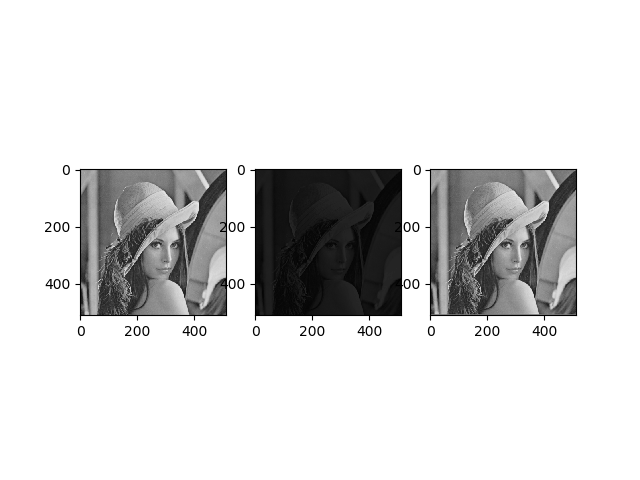
\includegraphics[scale=0.9]{Imagenes/E32S01}
\centering
\caption{Resultados caso $E=32$ $\sigma = 1$ }
\end{figure}
 
\begin{figure}
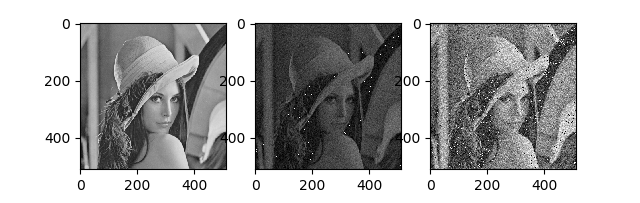
\includegraphics[scale=0.9]{Imagenes/E32S10}
\centering
\caption{Resultados caso $E=32$ $\sigma = 10$ }
\end{figure}

\begin{figure}
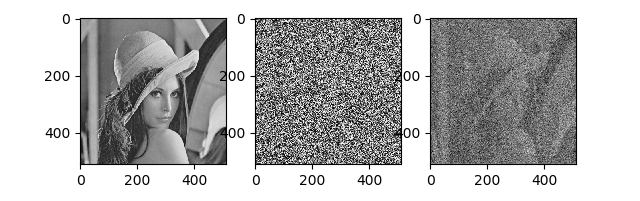
\includegraphics[scale=0.9]{Imagenes/E32S100}
\centering
\caption{Resultados caso $E=32$ $\sigma = 100$ }
\end{figure}

\begin{figure}
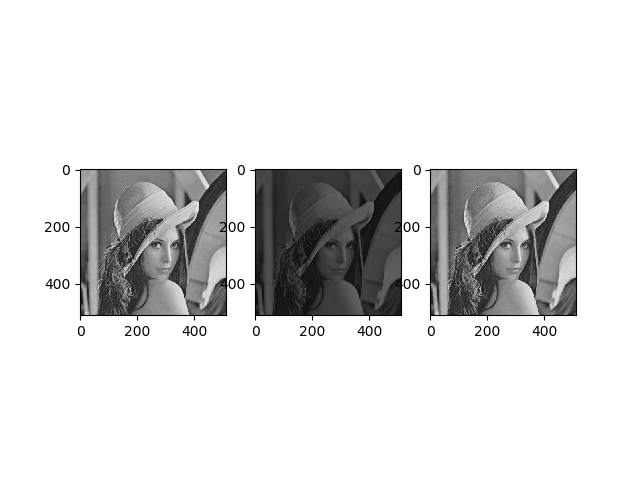
\includegraphics[scale=0.9]{Imagenes/E1024S01}
\centering
\caption{Resultados caso $E=1024$ $\sigma = 1$ }
\end{figure}

\begin{figure}
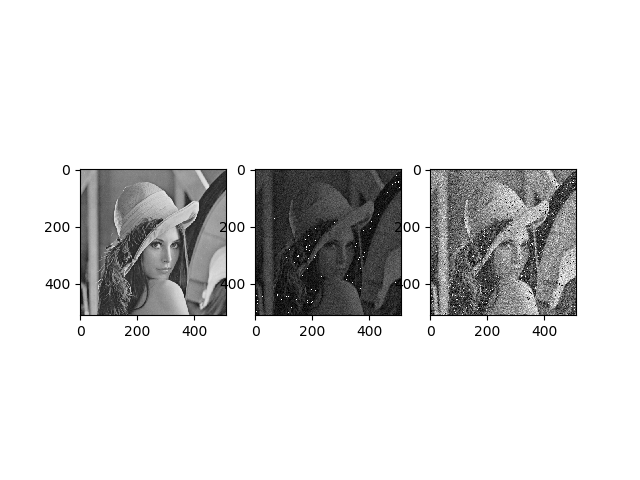
\includegraphics[scale=0.9]{Imagenes/E1024S10}
\centering
\caption{Resultados caso $E=1024$ $\sigma = 10$ }
\end{figure}

\begin{figure}
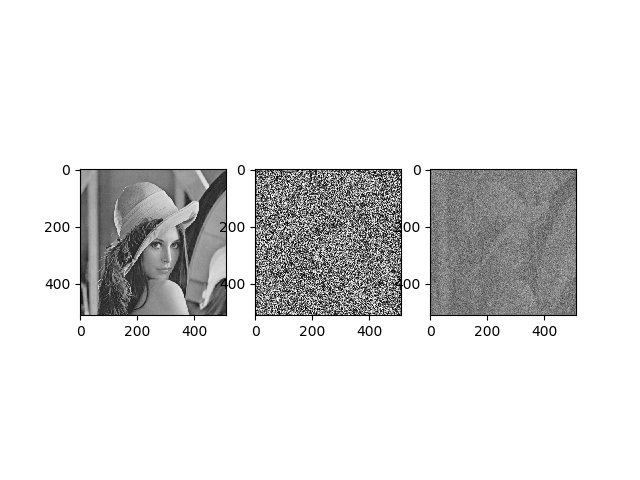
\includegraphics[scale=0.9]{Imagenes/E1024S100}
\centering
\caption{Resultados caso $E=1024$ $\sigma = 100$ }
\end{figure}

%\end{document}
